%% template.tex
%% from
%% bare_conf.tex
%% V1.4b
%% 2015/08/26
%% by Michael Shell
%% See:
%% http://www.michaelshell.org/
%% for current contact information.
%%
%% This is a skeleton file demonstrating the use of IEEEtran.cls
%% (requires IEEEtran.cls version 1.8b or later) with an IEEE
%% conference paper.
%%
%% Support sites:
%% http://www.michaelshell.org/tex/ieeetran/
%% http://www.ctan.org/pkg/ieeetran
%% and
%% http://www.ieee.org/

%%*************************************************************************
%% Legal Notice:
%% This code is offered as-is without any warranty either expressed or
%% implied; without even the implied warranty of MERCHANTABILITY or
%% FITNESS FOR A PARTICULAR PURPOSE!
%% User assumes all risk.
%% In no event shall the IEEE or any contributor to this code be liable for
%% any damages or losses, including, but not limited to, incidental,
%% consequential, or any other damages, resulting from the use or misuse
%% of any information contained here.
%%
%% All comments are the opinions of their respective authors and are not
%% necessarily endorsed by the IEEE.
%%
%% This work is distributed under the LaTeX Project Public License (LPPL)
%% ( http://www.latex-project.org/ ) version 1.3, and may be freely used,
%% distributed and modified. A copy of the LPPL, version 1.3, is included
%% in the base LaTeX documentation of all distributions of LaTeX released
%% 2003/12/01 or later.
%% Retain all contribution notices and credits.
%% ** Modified files should be clearly indicated as such, including  **
%% ** renaming them and changing author support contact information. **
%%*************************************************************************


% *** Authors should verify (and, if needed, correct) their LaTeX system  ***
% *** with the testflow diagnostic prior to trusting their LaTeX platform ***
% *** with production work. The IEEE's font choices and paper sizes can   ***
% *** trigger bugs that do not appear when using other class files.       ***                          ***
% The testflow support page is at:
% http://www.michaelshell.org/tex/testflow/

\documentclass[conference,]{IEEEtran}
% Some Computer Society conferences also require the compsoc mode option,
% but others use the standard conference format.
%
% If IEEEtran.cls has not been installed into the LaTeX system files,
% manually specify the path to it like:
% \documentclass[conference]{../sty/IEEEtran}





% Some very useful LaTeX packages include:
% (uncomment the ones you want to load)


% *** MISC UTILITY PACKAGES ***
%
%\usepackage{ifpdf}
% Heiko Oberdiek's ifpdf.sty is very useful if you need conditional
% compilation based on whether the output is pdf or dvi.
% usage:
% \ifpdf
%   % pdf code
% \else
%   % dvi code
% \fi
% The latest version of ifpdf.sty can be obtained from:
% http://www.ctan.org/pkg/ifpdf
% Also, note that IEEEtran.cls V1.7 and later provides a builtin
% \ifCLASSINFOpdf conditional that works the same way.
% When switching from latex to pdflatex and vice-versa, the compiler may
% have to be run twice to clear warning/error messages.






% *** CITATION PACKAGES ***
%
%\usepackage{cite}
% cite.sty was written by Donald Arseneau
% V1.6 and later of IEEEtran pre-defines the format of the cite.sty package
% \cite{} output to follow that of the IEEE. Loading the cite package will
% result in citation numbers being automatically sorted and properly
% "compressed/ranged". e.g., [1], [9], [2], [7], [5], [6] without using
% cite.sty will become [1], [2], [5]--[7], [9] using cite.sty. cite.sty's
% \cite will automatically add leading space, if needed. Use cite.sty's
% noadjust option (cite.sty V3.8 and later) if you want to turn this off
% such as if a citation ever needs to be enclosed in parenthesis.
% cite.sty is already installed on most LaTeX systems. Be sure and use
% version 5.0 (2009-03-20) and later if using hyperref.sty.
% The latest version can be obtained at:
% http://www.ctan.org/pkg/cite
% The documentation is contained in the cite.sty file itself.






% *** GRAPHICS RELATED PACKAGES ***
%
\ifCLASSINFOpdf
  % \usepackage[pdftex]{graphicx}
  % declare the path(s) where your graphic files are
  % \graphicspath{{../pdf/}{../jpeg/}}
  % and their extensions so you won't have to specify these with
  % every instance of \includegraphics
  % \DeclareGraphicsExtensions{.pdf,.jpeg,.png}
\else
  % or other class option (dvipsone, dvipdf, if not using dvips). graphicx
  % will default to the driver specified in the system graphics.cfg if no
  % driver is specified.
  % \usepackage[dvips]{graphicx}
  % declare the path(s) where your graphic files are
  % \graphicspath{{../eps/}}
  % and their extensions so you won't have to specify these with
  % every instance of \includegraphics
  % \DeclareGraphicsExtensions{.eps}
\fi
% graphicx was written by David Carlisle and Sebastian Rahtz. It is
% required if you want graphics, photos, etc. graphicx.sty is already
% installed on most LaTeX systems. The latest version and documentation
% can be obtained at:
% http://www.ctan.org/pkg/graphicx
% Another good source of documentation is "Using Imported Graphics in
% LaTeX2e" by Keith Reckdahl which can be found at:
% http://www.ctan.org/pkg/epslatex
%
% latex, and pdflatex in dvi mode, support graphics in encapsulated
% postscript (.eps) format. pdflatex in pdf mode supports graphics
% in .pdf, .jpeg, .png and .mps (metapost) formats. Users should ensure
% that all non-photo figures use a vector format (.eps, .pdf, .mps) and
% not a bitmapped formats (.jpeg, .png). The IEEE frowns on bitmapped formats
% which can result in "jaggedy"/blurry rendering of lines and letters as
% well as large increases in file sizes.
%
% You can find documentation about the pdfTeX application at:
% http://www.tug.org/applications/pdftex

\usepackage{graphicx}

% *** MATH PACKAGES ***
%
\usepackage{amsmath}
\usepackage{amssymb}
\interdisplaylinepenalty=2500
%\usepackage{amsmath}
% A popular package from the American Mathematical Society that provides
% many useful and powerful commands for dealing with mathematics.
%
% Note that the amsmath package sets \interdisplaylinepenalty to 10000
% thus preventing page breaks from occurring within multiline equations. Use:
%\interdisplaylinepenalty=2500
% after loading amsmath to restore such page breaks as IEEEtran.cls normally
% does. amsmath.sty is already installed on most LaTeX systems. The latest
% version and documentation can be obtained at:
% http://www.ctan.org/pkg/amsmath





% *** SPECIALIZED LIST PACKAGES ***
%
%\usepackage{algorithmic}
% algorithmic.sty was written by Peter Williams and Rogerio Brito.
% This package provides an algorithmic environment fo describing algorithms.
% You can use the algorithmic environment in-text or within a figure
% environment to provide for a floating algorithm. Do NOT use the algorithm
% floating environment provided by algorithm.sty (by the same authors) or
% algorithm2e.sty (by Christophe Fiorio) as the IEEE does not use dedicated
% algorithm float types and packages that provide these will not provide
% correct IEEE style captions. The latest version and documentation of
% algorithmic.sty can be obtained at:
% http://www.ctan.org/pkg/algorithms
% Also of interest may be the (relatively newer and more customizable)
% algorithmicx.sty package by Szasz Janos:
% http://www.ctan.org/pkg/algorithmicx




% *** ALIGNMENT PACKAGES ***
%
%\usepackage{array}
% Frank Mittelbach's and David Carlisle's array.sty patches and improves
% the standard LaTeX2e array and tabular environments to provide better
% appearance and additional user controls. As the default LaTeX2e table
% generation code is lacking to the point of almost being broken with
% respect to the quality of the end results, all users are strongly
% advised to use an enhanced (at the very least that provided by array.sty)
% set of table tools. array.sty is already installed on most systems. The
% latest version and documentation can be obtained at:
% http://www.ctan.org/pkg/array


% IEEEtran contains the IEEEeqnarray family of commands that can be used to
% generate multiline equations as well as matrices, tables, etc., of high
% quality.




% *** SUBFIGURE PACKAGES ***
%\ifCLASSOPTIONcompsoc
%  \usepackage[caption=false,font=normalsize,labelfont=sf,textfont=sf]{subfig}
%\else
%  \usepackage[caption=false,font=footnotesize]{subfig}
%\fi
% subfig.sty, written by Steven Douglas Cochran, is the modern replacement
% for subfigure.sty, the latter of which is no longer maintained and is
% incompatible with some LaTeX packages including fixltx2e. However,
% subfig.sty requires and automatically loads Axel Sommerfeldt's caption.sty
% which will override IEEEtran.cls' handling of captions and this will result
% in non-IEEE style figure/table captions. To prevent this problem, be sure
% and invoke subfig.sty's "caption=false" package option (available since
% subfig.sty version 1.3, 2005/06/28) as this is will preserve IEEEtran.cls
% handling of captions.
% Note that the Computer Society format requires a larger sans serif font
% than the serif footnote size font used in traditional IEEE formatting
% and thus the need to invoke different subfig.sty package options depending
% on whether compsoc mode has been enabled.
%
% The latest version and documentation of subfig.sty can be obtained at:
% http://www.ctan.org/pkg/subfig




% *** FLOAT PACKAGES ***
%

%\usepackage{fixltx2e}
% fixltx2e, the successor to the earlier fix2col.sty, was written by
% Frank Mittelbach and David Carlisle. This package corrects a few problems
% in the LaTeX2e kernel, the most notable of which is that in current
% LaTeX2e releases, the ordering of single and double column floats is not
% guaranteed to be preserved. Thus, an unpatched LaTeX2e can allow a
% single column figure to be placed prior to an earlier double column
% figure.
% Be aware that LaTeX2e kernels dated 2015 and later have fixltx2e.sty's
% corrections already built into the system in which case a warning will
% be issued if an attempt is made to load fixltx2e.sty as it is no longer
% needed.
% The latest version and documentation can be found at:
% http://www.ctan.org/pkg/fixltx2e


%\usepackage{stfloats}
% stfloats.sty was written by Sigitas Tolusis. This package gives LaTeX2e
% the ability to do double column floats at the bottom of the page as well
% as the top. (e.g., "\begin{figure*}[!b]" is not normally possible in
% LaTeX2e). It also provides a command:
%\fnbelowfloat
% to enable the placement of footnotes below bottom floats (the standard
% LaTeX2e kernel puts them above bottom floats). This is an invasive package
% which rewrites many portions of the LaTeX2e float routines. It may not work
% with other packages that modify the LaTeX2e float routines. The latest
% version and documentation can be obtained at:
% http://www.ctan.org/pkg/stfloats
% Do not use the stfloats baselinefloat ability as the IEEE does not allow
% \baselineskip to stretch. Authors submitting work to the IEEE should note
% that the IEEE rarely uses double column equations and that authors should try
% to avoid such use. Do not be tempted to use the cuted.sty or midfloat.sty
% packages (also by Sigitas Tolusis) as the IEEE does not format its papers in
% such ways.
% Do not attempt to use stfloats with fixltx2e as they are incompatible.
% Instead, use Morten Hogholm'a dblfloatfix which combines the features
% of both fixltx2e and stfloats:
%
% \usepackage{dblfloatfix}
% The latest version can be found at:
% http://www.ctan.org/pkg/dblfloatfix




% *** PDF, URL AND HYPERLINK PACKAGES ***
%
%\usepackage{url}
% url.sty was written by Donald Arseneau. It provides better support for
% handling and breaking URLs. url.sty is already installed on most LaTeX
% systems. The latest version and documentation can be obtained at:
% http://www.ctan.org/pkg/url
% Basically, \url{my_url_here}.




% *** Do not adjust lengths that control margins, column widths, etc. ***
% *** Do not use packages that alter fonts (such as pslatex).         ***
% There should be no need to do such things with IEEEtran.cls V1.6 and later.
% (Unless specifically asked to do so by the journal or conference you plan
% to submit to, of course. )



%% BEGIN MY ADDITIONS %%

\usepackage[citestyle=ieee,,]{biblatex}
\addbibresource{bibliography.bib}

\usepackage[unicode=true]{hyperref}
\usepackage[noabbrev,capitalize]{cleveref}

\hypersetup{
            pdftitle={3D Point Cloud Reconstruction from UAV Images through Incremental Structure from Motion (SfM) for Plant Phenotyping},
            pdfkeywords={3D reconstruction, phenotyping, structure from
motion, incremental structure from motion, point cloud processing},
            pdfborder={0 0 0},
            breaklinks=true}
\urlstyle{same}  % don't use monospace font for urls

% Pandoc toggle for numbering sections (defaults to be off)
\setcounter{secnumdepth}{5}


% tightlist command for lists without linebreak
\providecommand{\tightlist}{%
  \setlength{\itemsep}{0pt}\setlength{\parskip}{0pt}}

% From pandoc table feature
\usepackage{longtable,booktabs,array}
\usepackage{calc} % for calculating minipage widths
% Correct order of tables after \paragraph or \subparagraph
\usepackage{etoolbox}
\makeatletter
\patchcmd\longtable{\par}{\if@noskipsec\mbox{}\fi\par}{}{}
\makeatother
% Allow footnotes in longtable head/foot
\IfFileExists{footnotehyper.sty}{\usepackage{footnotehyper}}{\usepackage{footnote}}
\makesavenoteenv{longtable}


\makeatletter
\makeatother
\makeatletter
\makeatother
\makeatletter
\@ifpackageloaded{caption}{}{\usepackage{caption}}
\AtBeginDocument{%
\ifdefined\contentsname
  \renewcommand*\contentsname{Table of contents}
\else
  \newcommand\contentsname{Table of contents}
\fi
\ifdefined\listfigurename
  \renewcommand*\listfigurename{List of Figures}
\else
  \newcommand\listfigurename{List of Figures}
\fi
\ifdefined\listtablename
  \renewcommand*\listtablename{List of Tables}
\else
  \newcommand\listtablename{List of Tables}
\fi
\ifdefined\figurename
  \renewcommand*\figurename{Figure}
\else
  \newcommand\figurename{Figure}
\fi
\ifdefined\tablename
  \renewcommand*\tablename{Table}
\else
  \newcommand\tablename{Table}
\fi
}
\@ifpackageloaded{float}{}{\usepackage{float}}
\floatstyle{ruled}
\@ifundefined{c@chapter}{\newfloat{codelisting}{h}{lop}}{\newfloat{codelisting}{h}{lop}[chapter]}
\floatname{codelisting}{Listing}
\newcommand*\listoflistings{\listof{codelisting}{List of Listings}}
\makeatother
\makeatletter
\@ifpackageloaded{caption}{}{\usepackage{caption}}
\@ifpackageloaded{subcaption}{}{\usepackage{subcaption}}
\makeatother
\makeatletter
\@ifpackageloaded{tcolorbox}{}{\usepackage[skins,breakable]{tcolorbox}}
\makeatother
\makeatletter
\@ifundefined{shadecolor}{\definecolor{shadecolor}{rgb}{.97, .97, .97}}
\makeatother
\makeatletter
\makeatother
\makeatletter
\makeatother

%% END MY ADDITIONS %%


\hyphenation{}

\begin{document}
%
% paper title
% Titles are generally capitalized except for words such as a, an, and, as,
% at, but, by, for, in, nor, of, on, or, the, to and up, which are usually
% not capitalized unless they are the first or last word of the title.
% Linebreaks \\ can be used within to get better formatting as desired.
% Do not put math or special symbols in the title.
\title{3D Point Cloud Reconstruction from UAV Images through Incremental
Structure from Motion (SfM) for Plant Phenotyping}

% author names and affiliations
% use a multiple column layout for up to three different
% affiliations

\author{

%% ---- classic IEEETrans wide authors' list ----------------

%% ----------------------------------------------------------

%% ---- classic IEEETrans one column per institution --------
 %%
%% ----------------------------------------------------------





%% ---- one column per author, classic/default IEEETrans ----
\IEEEauthorblockN{Andreas Ming}
\IEEEauthorblockA{
\textit{Institute of Electrical Engineering}\\
\textit{Lucerne University of Applied Sciences and Arts}\\
\textit{Horw, Switzerland}
\\andreas.ming@stud.hslu.ch
%%
}

\and
\IEEEauthorblockN{Richard Green}
\IEEEauthorblockA{
\textit{Department of Computer Science and Software Engineering}\\
\textit{University of Canterbury}\\
\textit{Christchurch, New Zealand}
\\richard.green@canterbury.ac.nz
%%
}



%% ----------------------------------------------------------

}

% conference papers do not typically use \thanks and this command
% is locked out in conference mode. If really needed, such as for
% the acknowledgment of grants, issue a \IEEEoverridecommandlockouts
% after \documentclass

% for over three affiliations, or if they all won't fit within the width
% of the page, use this alternative format:
%
%\author{\IEEEauthorblockN{Michael Shell\IEEEauthorrefmark{1},
%Homer Simpson\IEEEauthorrefmark{2},
%James Kirk\IEEEauthorrefmark{3},
%Montgomery Scott\IEEEauthorrefmark{3} and
%Eldon Tyrell\IEEEauthorrefmark{4}}
%\IEEEauthorblockA{\IEEEauthorrefmark{1}School of Electrical and Computer Engineering\\
%Georgia Institute of Technology,
%Atlanta, Georgia 30332--0250\\ Email: see http://www.michaelshell.org/contact.html}
%\IEEEauthorblockA{\IEEEauthorrefmark{2}Twentieth Century Fox, Springfield, USA\\
%Email: homer@thesimpsons.com}
%\IEEEauthorblockA{\IEEEauthorrefmark{3}Starfleet Academy, San Francisco, California 96678-2391\\
%Telephone: (800) 555--1212, Fax: (888) 555--1212}
%\IEEEauthorblockA{\IEEEauthorrefmark{4}Tyrell Inc., 123 Replicant Street, Los Angeles, California 90210--4321}}




% use for special paper notices
%\IEEEspecialpapernotice{(Invited Paper)}




% make the title area
\maketitle

% As a general rule, do not put math, special symbols or citations
% in the abstract
\begin{abstract}
The paper proposed a method for constructing a 3D point cloud of plants
from overhead images taken by a unmanned aerial vehicle (UAV). The
structure-from motion (SfM) algorithm constructs a point cloud through
SIFT feature extraction, matching, and geometric verifications in
correspondence search, and next best view selection, triangulation,
local bundle adjustment, retriangulation, observation merging, and
global bundle adjustment in a incremental SfM approach. Comparing the
algorithm to a commercially available solution, shows that the
commercial solution generates 150\% more voxels. Furthermore, by
reconstructing the point cloud with the high resolution images and
finally applying multi-view-stereo (MVS) for point cloud densification,
950\% and 9000\% more voxels are generated respectively. Future research
into incorporation of geolocation data, MVS, and deep learning
approaches like neural radiance fields (NeRF) for dense point cloud
reconstruction and real-time processing are recommended.
\end{abstract}

% keywords
\begin{IEEEkeywords}
3D reconstruction, phenotyping, structure from motion, incremental
structure from motion, point cloud processing
\end{IEEEkeywords}

% use for special paper notices



% make the title area
\maketitle

% no keywords

% For peer review papers, you can put extra information on the cover
% page as needed:
% \ifCLASSOPTIONpeerreview
% \begin{center} \bfseries EDICS Category: 3-BBND \end{center}
% \fi
%
% For peerreview papers, this IEEEtran command inserts a page break and
% creates the second title. It will be ignored for other modes.
\IEEEpeerreviewmaketitle

\ifdefined\Shaded\renewenvironment{Shaded}{\begin{tcolorbox}[sharp corners, interior hidden, boxrule=0pt, borderline west={3pt}{0pt}{shadecolor}, frame hidden, enhanced, breakable]}{\end{tcolorbox}}\fi


\hypertarget{introduction}{%
\section{Introduction}\label{introduction}}

To overcome the up to 56\% increase in food demand by 2050, serious
measures have to be applied, as current crop production is insufficient
to lower the risk of hunger. Furthermore, an overall more stable crop
production, able to deal with pests, pathogens, heat waves, and other
climate change induced weather extremes, must be achieved
\autocite{vandijk2021}. A key point of breeding new resilient crops are
double haploidy, genomics-assisted breeding, breeding data management,
and high-throughput and precise phenotyping
\autocite{prasanna2021,araus2018}. Acquisition of large-scale phenotype
data in traditional research is mainly based on manual measurements and
thus become a major bottleneck for big-data \autocite{yang2020}.
Unmanned areal vehicles (UAV) - drones are used in agriculture for
pesticide spraying and crop monitoring. Equipped with various sensors
and cameras of different spectra, drones are a useful tool for crop
monitoring, either for pesticide spraying, fertiliser estimation, or
crop monitoring \autocite{mogili2018}.

\begin{figure}

{\centering 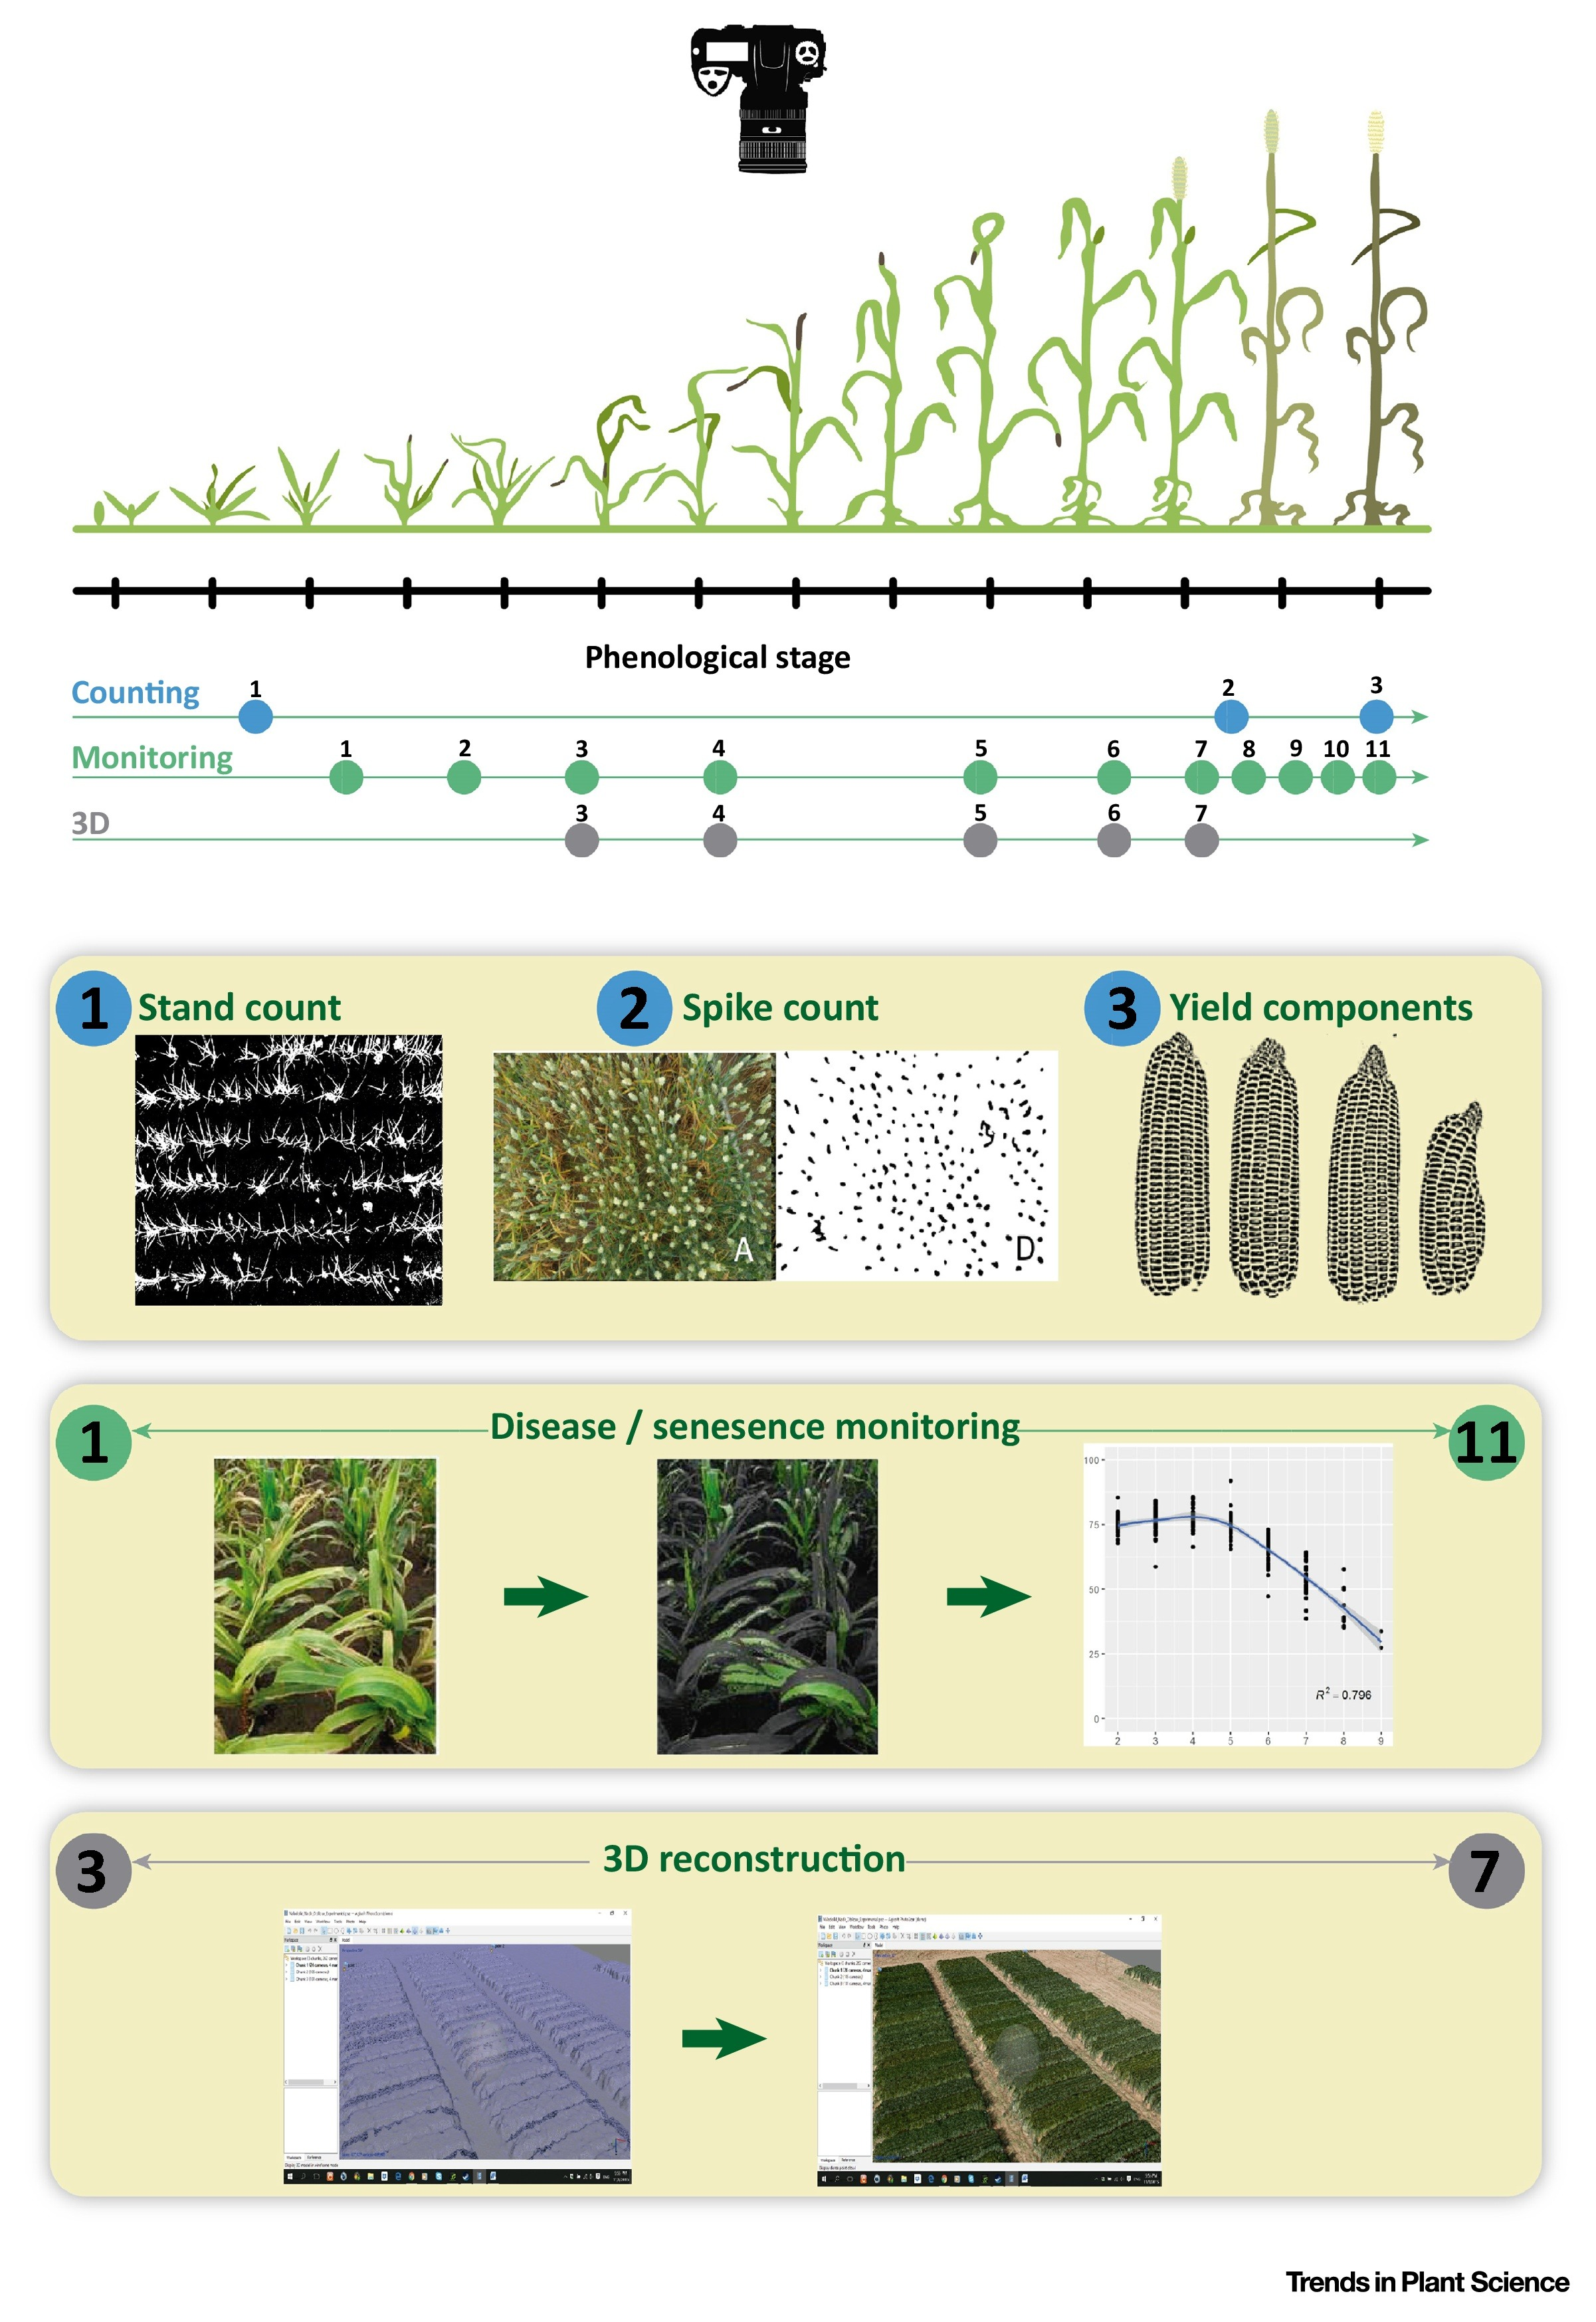
\includegraphics[width=8cm,height=11.5cm]{images/pheneostages.jpg}

}

\caption{\label{fig-pheneostages}Examples of potential applications of
field phenotyping with RGB-images. Different phenotyping needs in
respect to the corresponding pheneological stage. \autocite{araus2018}}

\end{figure}

In plant phenotyping specifically, there is a need in the accurate
capture of individual plants, or the recording of individual
characteristics depending on the phonological stage of a plant (see
Figure~\ref{fig-pheneostages}) \autocite{araus2018}. Traditionally
ground based systems are used for this task, as the environmental
variables can be controlled much easier \autocite{yang2020}. If drones
could be used instead, this would increase effectiveness and reduce the
direct environmental impact, e.g.~through ground pressure. Drones seam
to be especially useful for this task, based on the low price and
ease-of-use \autocite{guo2021}. If needed, drones can be combined with
ground robots to capture more data from angles obstructed for the drone
(e.g.~under the canopy) \autocite{gao2021}. 3D reconstruction is a
important part of phenotyping, and if accurate enough, could work as a
new base for algorithms to work out other plant details like
correlations between biomass and plant constituents \autocite{xiao2020}.
Furthermore, with the acquisition of precise 3D models of plants over
time, functional structural plant models (FSPMs) can be constructed and
conclusions drawn \autocite{soualiou2021}.

3D reconstruction through Structure-from-Motion (SfM) is usually
featured as lightweight and cheap to implement, as just one or more
standard monochrome or colour cameras need to be used to capture the
desired images. Furthermore, a complete reconstruction can be done on
unstructured images, without the use of references e.g.~global
navigation satellite system (GNSS). With increasing dataset size a
higher resolution can be achieved and SfM algorithms are typically able
to provide mm-accuracy \autocite{paulus2019}.

\hypertarget{sec-background}{%
\section{Background}\label{sec-background}}

This section describes the state-of-the-art implementation of SfM for 3D
reconstruction and is heavily based on J.~Schönebergers
\autocite{schönberger2016,schönberger2016a} work, and the implementation
in COLMAPS \autocite{schönberger2024}.

SfM is constructing a scene through projections of images taken from
different viewpoints. To incorporate a series of images, a sequential
processing pipeline with a iterative reconstruction component forms the
incremental SfM (see \cref{fig-recons_algo}). \autocite{schönberger2016}

After completing the iterative SfM, we acquired a set of poses
\(\mathcal{P}\) and reconstructed points \(\mathcal{X}\). These points
\(X_k\) represent the triangulation of matched key points between image
pairs.

\begin{figure*}[htbp]
\centering
\includegraphics[width=\textwidth]{images/recons_algo.png}
\caption{Incremental SfM pipeline (adapted from \autocite{schönberger2016})}
\label{fig-recons_algo}
\end{figure*}

\hypertarget{correspondence-search}{%
\subsection{Correspondence Search}\label{correspondence-search}}

The first stage identifies projections of the same points in overlapping
input images (key points) and then outputs a set of geometrically
verified image pairs as well as a graph of the image projections for
each point. \autocite{schönberger2016}

\hypertarget{feature-extraction}{%
\subsubsection{Feature Extraction}\label{feature-extraction}}

For each input image \(I_i\), sets of local features
\(\mathcal{F}_i=\{(x_j,f_j)|j=1\dots N_{F_i}\}\) represented as a
appearance descriptor \(f_j\) at location \(x_j\in \mathbb{R}^2\) are
processed. To be uniquely recognisable in different images, the features
should be invariant under radiometric and geometric changes
\autocite{mcglone2004}. Several feature detectors based of Scale
Invariant Feature Transform (SIFT) \autocite{lowe1999,tuytelaars2008}
appear to be especially performing in terms of robustness.
\autocite{schönberger2016}

\hypertarget{matching}{%
\subsubsection{Matching}\label{matching}}

To work out scene overlaps between images for later triangulation, the
features \(\mathcal{F}_j\) of all image pairs are tested. It searches
for corresponding features by finding the most similar feature in image
\(I_a\) for each feature in image \(I_b\) through the similarity metric
\(f_j\). The output of this are potential overlapping image pairs
\(\mathcal{C}=\{I_a,I_b\}\) and their respective feature correspondences
\(\mathcal{M}_{ab}\).\autocite{schönberger2016}

\hypertarget{geometric-verification}{%
\subsubsection{Geometric Verification}\label{geometric-verification}}

Since matching is only based on appearance and not location, it can not
be guaranteed that the potential image pairs \(\mathcal{C}\) are
actually overlapping. To verify this, SfM estimates a transformation
matrix that maps feature points between images. As a result, a
homography \(\mathbf{H}\) for planar scenes, a essential matrix
\(\mathbf{E}\), or a fundamental matrix \(\mathbf{F}\) for moving
cameras is estimated. Because of heavy outlier-contaminated matching
correspondences, robust estimators like RANSAC \autocite{fischler1981}
are required. A potential image pair \(\mathcal{C}\) becomes a verified
image pair \(\bar{\mathcal{C}}\) if enough inliers can be described as a
fundamental matrix \(\mathbf{F}\). Besides the verified image pair
\(\bar{\mathcal{C}}\), their respective inlier correspondence
\(\bar{\mathcal{M}}_{ab}\), and a description of their geometric
relation \(\mathcal{G}_{ab}\) are outputted by this stage. To compute
the geometric relation \(\mathcal{G}_{ab}\), GRIC \autocite{torr1997} is
used as a decision criterion. The output of GRIC is a scene graph with
images as nodes and verified pairs of images as edges.
\autocite{schönberger2016}

\hypertarget{incremental-reconstruction}{%
\subsection{Incremental
Reconstruction}\label{incremental-reconstruction}}

The reconstruction stage computes the pose estimates \(\mathcal{P}\) and
the reconstructed scene as a set of points \(\mathcal{X}\) with
\(X_k\in\mathbb{R}^3\). For that, the scene graph from the last scene is
used and one image after the other is added to the model. In a iterative
process, all images are incorporated in the reconstruction of the scene.
\autocite{schönberger2016}

\hypertarget{next-best-view-selection}{%
\subsubsection{Next Best View
Selection}\label{next-best-view-selection}}

To work out what images to take next, and especially with what pair of
images to start with, a robust view selection has to be applied. This is
done through a scoring approach which is applied to each image, more
precisely to the matching key points of image pairs. More visible points
and a more uniform distribution of these points results in a higher
score \(\mathcal{S}\) (see Figure~\ref{fig-BestViewSelection})
\autocite{irschara2009}. Because of more points to triangulate, images
with a high score are, especially in early iterations, better suited for
a robust reconstruction.

\begin{figure}

{\centering 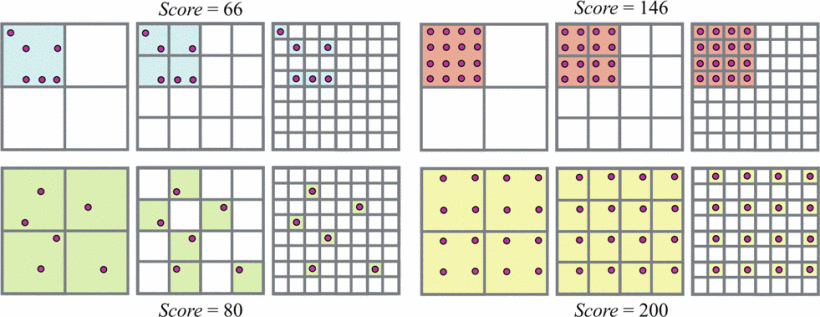
\includegraphics[width=8.5cm,height=3.3cm]{images/BestViewSelection.png}

}

\caption{\label{fig-BestViewSelection}Scores for different number of
points (left and right) with different distributions (top and bottom) in
the image for \(L=3\) \autocite{schönberger2016}}

\end{figure}

Each image is split into a grid of cells which are either \emph{empty}
if no point is present, or \emph{full} if one or more points are
present. This gives a higher score to equally distributed points. This
scheme might not capture distribution well if few partitions are
present, as every partition might be activated by a point (e.g.~most
bottom left configuration in Figure~\ref{fig-BestViewSelection}).
Therefore a multi resolution approach with \(l=1\dots L\) levels of
partitioning with incrementing resolution \(K_l=2^l\) is used. The score
is then accumulated over all levels. \autocite{schönberger2016}

\hypertarget{image-registration}{%
\subsubsection{Image Registration}\label{image-registration}}

Through the Next Best View Selection approach, we get the image which
sees the most triangulated points of the current model. To estimate the
pose \(\mathbf{P}_c\) of the newly registered image, we further maximise
the score and thus the viewable points. This is commonly known as the
Perspective-n-Pose (PnP) \autocite{fischler1981} problem. The estimated
pose \(\mathbf{P}_c\) is then added to the set of poses \(\mathcal{P}\).
\autocite{schönberger2016}

\hypertarget{triangulation}{%
\subsubsection{Triangulation}\label{triangulation}}

With the registered image and the scene graph of the newly present image
pairs, further points \(X_k\) can be triangulated and added to the scene
set \(\mathcal{X}\). This point \(X_k\) is valid as soon as one or more
images covering the scene from a different viewpoint are registered. For
multi-view triangulation, and especially handling outlier contamination,
RANSAC is used. A feature track \(\mathcal{T}\) consisting of normalised
image observations \(\bar{x}_n\in\mathbb{R}^2\) and a corresponding pose
\(\mathbf{P}_n\). The goal is then to maximise the support of
measurements conforming with a triangulation

\[
X_{ab}\sim \tau(\bar{x}_a,\bar{x}_b,\mathbf{P}_a,\mathbf{P}_b)\text{ with } a\neq b
\]

where \(\tau\) is the DLT \autocite{hartley2004} triangulation method
and \(X_{ab}\) the triangulated point. A well-conditioned model
satisfies a sufficient triangulation angle \(\alpha\) and positive
depths \(d_{a/b}\) with respect to the image poses \(\mathbf{P}_{a/b}\).
\autocite{schönberger2016}

\hypertarget{local-bundle-adjustment}{%
\subsubsection{Local Bundle Adjustment}\label{local-bundle-adjustment}}

As image registration and triangulation are separate processes, their
outputs are highly correlated. Still there are uncertainties propagating
from camera poses to triangulation and similarly the reverse is true. To
further suppress such induced errors, we perform bundle adjustment.
Because incremental SfM affects models only locally, we only perform a
local BA on a set of the most connected images. BA is a iterative
process, with the goal to reduce a loss-function, in our case a Cauchy
function \(\rho_j\). The optimisation is performed through a Ceres
Solver \autocite{ceresso}. \autocite{schönberger2016}

\hypertarget{filtering}{%
\subsubsection{Filtering}\label{filtering}}

After a local BA, observations which do not conform with the model are
filtered out. These are characterised through a large reprojection error
\autocite{wu2013}. \autocite{schönberger2016}

\hypertarget{retirangulation}{%
\subsubsection{Retirangulation}\label{retirangulation}}

To account for drift effects induced through the local BA, a
retriangulation is performed. This helps in improving completeness of
reconstruction by continuing tracks of points, that previously might
have failed to triangulate. \autocite{schönberger2016}

\hypertarget{global-bundle-adjustment}{%
\subsubsection{Global Bundle
Adjustment}\label{global-bundle-adjustment}}

After the model has grown by a certain percentage, a global BA is
performed, resulting in a amortised linear run-time of SfM. Without this
refinement, SfM tend to drift into a non-recoverable state. Similarly,
to the local BA, a Cauchy function \(\rho_j\) is optimised with the
Ceres Solver \autocite{ceresso}. \autocite{schönberger2016}

\hypertarget{proposed-method}{%
\section{Proposed Method}\label{proposed-method}}

This section describes the proposed method for 3D reconstruction of
plants through a UAV for phenotyping. First, the imaging platform, which
consists of a drone equipped with a high resolution camera for imaging
the plants; second, the computer vision system, which builds a 3D point
cloud of the ground and its plants.

\hypertarget{sec-drone}{%
\subsection{Drone Platform}\label{sec-drone}}

As a basis for SfM reconstruction a series of pictures acquired by a
Drone with a built-in synchronised camera and RTK-GNSS System is used,
the dataset is publicly available by ref. \autocite{matsuura2023}. The
camera and RTK-GNSS are synchronised by a microcomputer on the drone
(see \cref{fig-DroneSetup}), while the images and their positions are
monitored from the ground base. The RTK-GNSS data is not used for 3D
reconstruction in this paper. For evaluation of the algorithm, a fake
plant, and three boxes of known size are placed on the ground, one of
the boxes with a plant on it. \autocite{matsuura2023}

\begin{figure*}[tp]
\centering
\subfloat{\includegraphics[width=3in]{images/drone.png}%
\label{fig-first_drone}}
\hfil
\subfloat{\includegraphics[width=3in]{images/testsetup.png}%
\label{fig-second_drone}}
\caption{Drone used to acquire the data (left) and the drone in the testing environment (right) \autocite{matsuura2023}}
\label{fig-DroneSetup}
\end{figure*}

Images are captured in a resolution of \(5472\) x \(3638\) pixels from a
height of \(10m\) and \(20m\) in a overflight configuration. For the
further drone specifications, refer to \cref{table_specs}.
\autocite{matsuura2023}

% ------------- Drone specs table -------------
\begin{table}
    \renewcommand{\arraystretch}{1.3}
    \caption{Drone Specifications \autocite{matsuura2023}}
    \label{table_specs}
    \centering
    \begin{tabular}{|>{\raggedright}p{0.35\linewidth}|p{0.55\linewidth}|}
        \hline
        \textbf{Component} & \textbf{Specification}\\
        \hline
        Drone Body & GD-X8 V2 (1000 mm)\\
        \hline
        Motors & T-motor P60 × 4 \\
        \hline
        Flight Controller & CUAV X7 \\
        \hline
        GNSS & RTK-GNSS: ZED-F9P module \\
        \hline
        Gimbal & GREMSY S1V3 \\
        \hline
        Camera & Canon PowerShot G7 X Mark 2 \\
        \hline
        Image Resolution & 5472 x 3638\\
        \hline
        Micro-computer & JETSON Nano \\
        \hline
    \end{tabular}
\end{table}

\hypertarget{computer-vision-system}{%
\subsection{Computer Vision System}\label{computer-vision-system}}

To retrieve a 3D point cloud for phenotyping of plants, we propose the
use of a incremental SfM approach as described in
Section~\ref{sec-background}. Due to computational limits (see
\cref{table_system_specs} for system specifications), images are
restricted to a resolution of \(2472\) x \(1648\). A comparison with a
commercially available 3D reconstruction tool PIX4Dmapper, utilising the
full resolution images, is done. Furthermore, the reconstruction with
PIX4Dmapper incorporates multi-view stereo (MVS) to further condense the
point cloud.

% ------------- System specs table -------------
\begin{table}
    \renewcommand{\arraystretch}{1.3}
    \caption{System Specifications}
    \label{table_system_specs}
    \centering
    \begin{tabular}{|>{\raggedright}p{0.35\linewidth}|p{0.55\linewidth}|}
        \hline
        \textbf{Component} & \textbf{Specification}\\
        \hline
        OS & Linux Mint 21.1 Cinnamon\\
        \hline
        CPU & 12$^{\text{th}}$ Gen Intel Core\texttrademark\space i7-12700x12\\
        \hline
        IDE & Visual Studio Code\\
        \hline
        Interpreter & Python 3.10.6\\
        \hline
        CUDA Support & No\\
        \hline
        Image Resolution & 2472 x 1648\\
        \hline
        COLMAP Version & 3.9.1\\
        \hline
    \end{tabular}
\end{table}

\hypertarget{sec-results}{%
\section{Results}\label{sec-results}}

The reconstruction algorithm is run on a system defined in
\cref{table_system_specs}. The algorithm is run on the downsampled
dataset acquired with the drone platform described in
Section~\ref{sec-drone}. All images are collected in one run and than
given to the algorithm as a unordered dataset. The algorithm then worked
out a 3D point cloud. For comparison, a 3D reconstruction with the
commercially available PIX4Dmapper is done on the downsampled and
original datasets. Additionally, a densification of the point cloud
through MVS is done in PIX4Dmapper on the high resolution data set.

If we compare the number of points in each point cloud in
\cref{tab-tool_performance}, it can be observed, that simple incremental
SfM produces the least amount of points, whereas PIX4Dmapper works out
150\% more points on the same dataset. With a higher resolution the
increase grows to 950\% and 9000\% if MVS is applied.

\begin{table}
    \renewcommand{\arraystretch}{1.3}
    \caption{Tool Performance}
    \label{tab-tool_performance}
    \centering
    \begin{tabular}{|>{\raggedright}p{0.55\linewidth}|p{0.35\linewidth}|}
        \hline
        \textbf{Tool} & \textbf{Reconstructed Points} \\
        \hline
        COLMAP (SfM, Low-Res) & 85749 \\
        \hline
        PIX4Dmapper (SfM, Low-Res) & 217153 \\
        \hline
        PIX4Dmapper (SfM, High-Res) & 901223 \\
        \hline
        PIX4Dmapper (SfM+MVS, High-Res) & 7859904 \\
        \hline
    \end{tabular}
\end{table}

\begin{figure*}[tp]
    \centering
    \subfloat[]{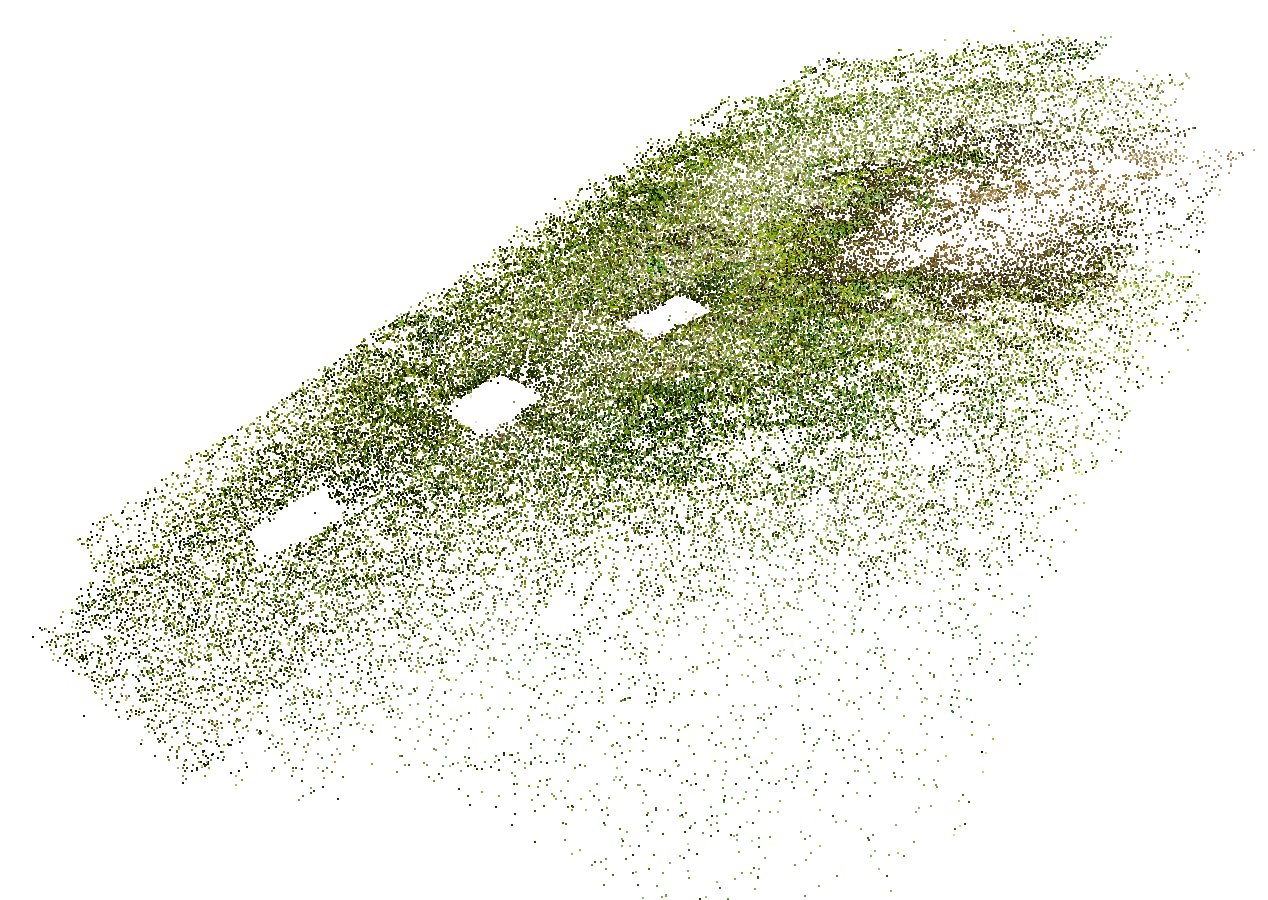
\includegraphics[width=0.25\textwidth]{images/pcd_clr_colmap.png}%
    \label{fig-colmap_clr}}
    \hfil
    \subfloat[]{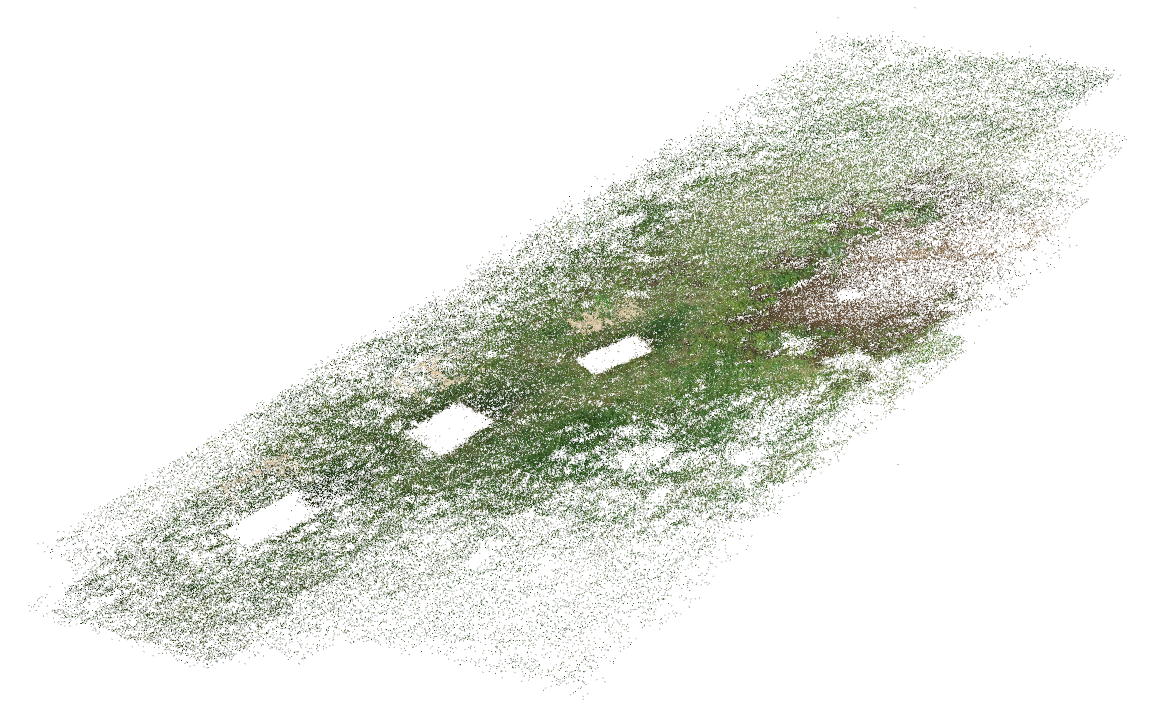
\includegraphics[width=0.25\textwidth]{images/pcd_clr_pix4d_ties.png}%
    \label{fig-pix4d_ties_lowres}}
    \hfil
    \subfloat[]{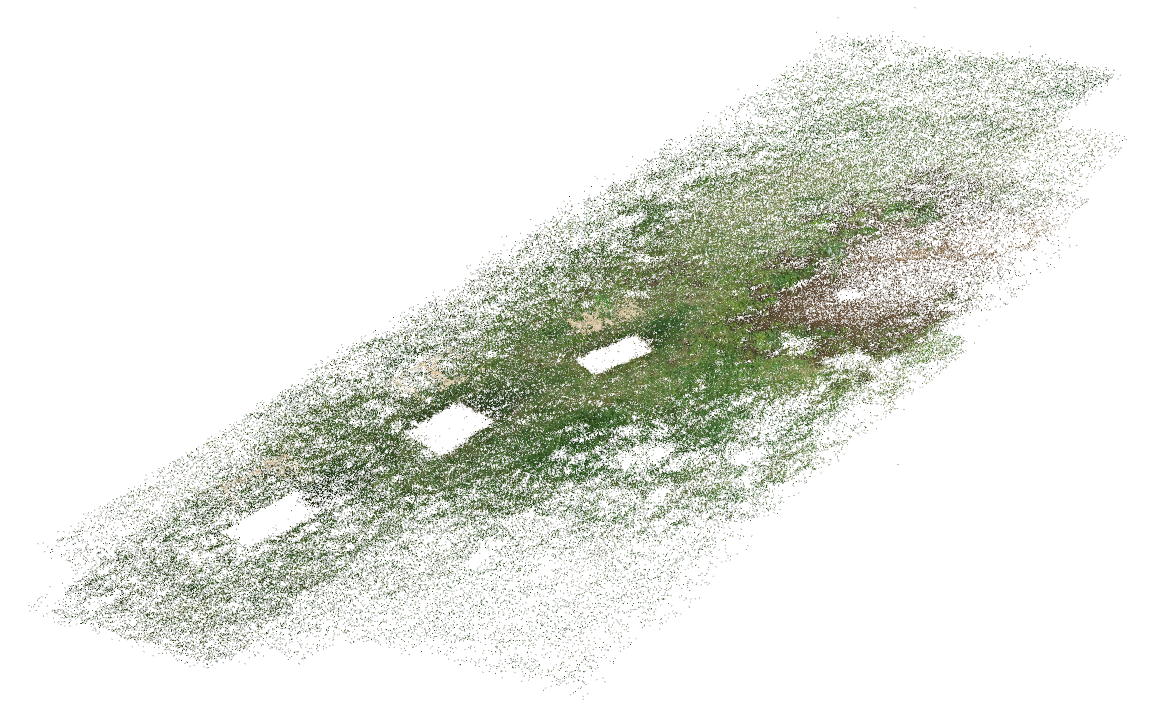
\includegraphics[width=0.25\textwidth]{images/pcd_clr_pix4d_ties.png}%
    \label{fig-pix4d_ties}}
    \hfil
    \subfloat[]{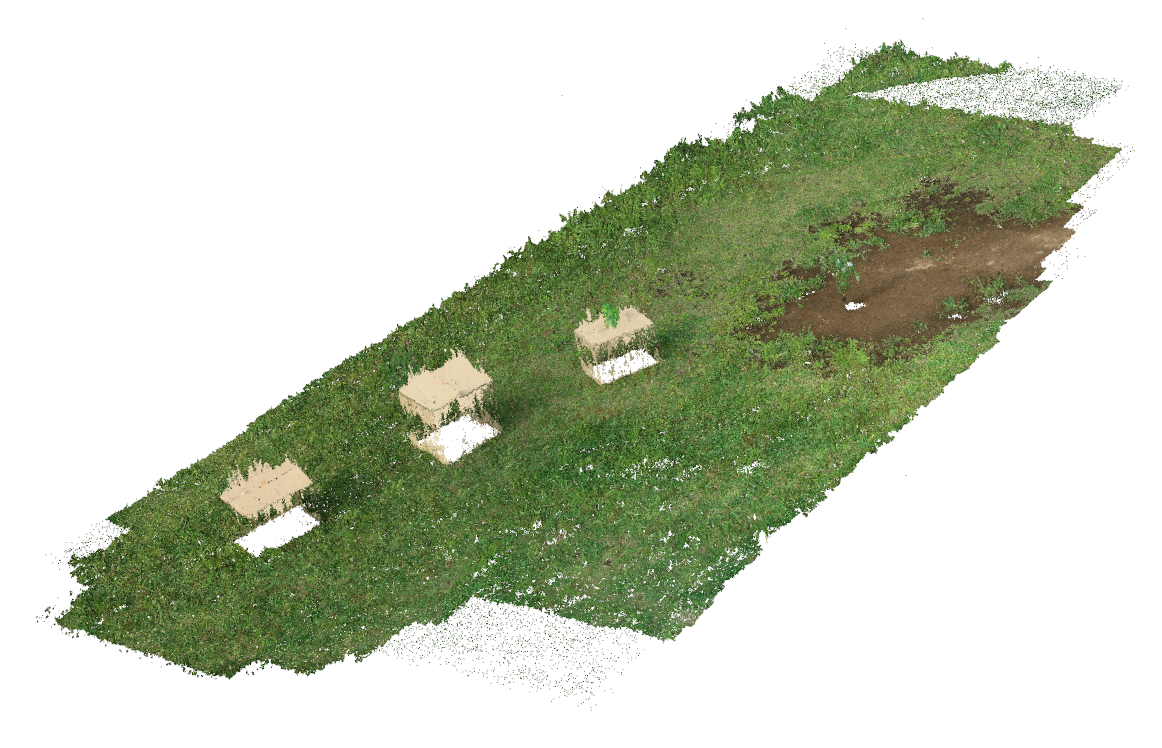
\includegraphics[width=0.25\textwidth]{images/pcd_clr_pix4d_stereo.png}%
    \label{fig-pix4d_stereo}}
    \caption{The reconstructed point clouds. In (a) through incremental SfM described in \cref{sec-background}, visualised in Open3D, (b) and (c) are computed with the commercial PIX4Dmapper and shows all triangulated points from matched image features (ties) on a low- and high-resolution dataset, respectively. In (d) MVS is applied in PIX4Dmapper for a denser point cloud.}
    \label{fig-pclouds}
\end{figure*}

To work out the plant heights, a peak finding algorithm is used. For
this, the point cloud is filtered for outliers, and a plane is fitted to
represent the ground. To find the plants, the point furthest away from
the plane is taken, and its surrounding points deleted for the next
iteration. This is repeated until the height falls under a certain
threshold. As seen in \cref{fig-plants}, bounding boxes are set around
each found peak, to visualise the separate plants in the point cloud. It
has been identified, that this algorithm can not distinguish between
plants, ground, nor different objects, as no segmentation is performed.
The algorithm is also incapable of adapting to different plant sizes, as
the bounding boxes are a fixed size. Furthermore, fitting the ground to
the plane leads to bumps in the ground to be recognised as plants. The
plane approximation only works for flat grounds or flat patches in
bigger point clouds.

\begin{figure*}[tp]
    \centering
    \subfloat[]{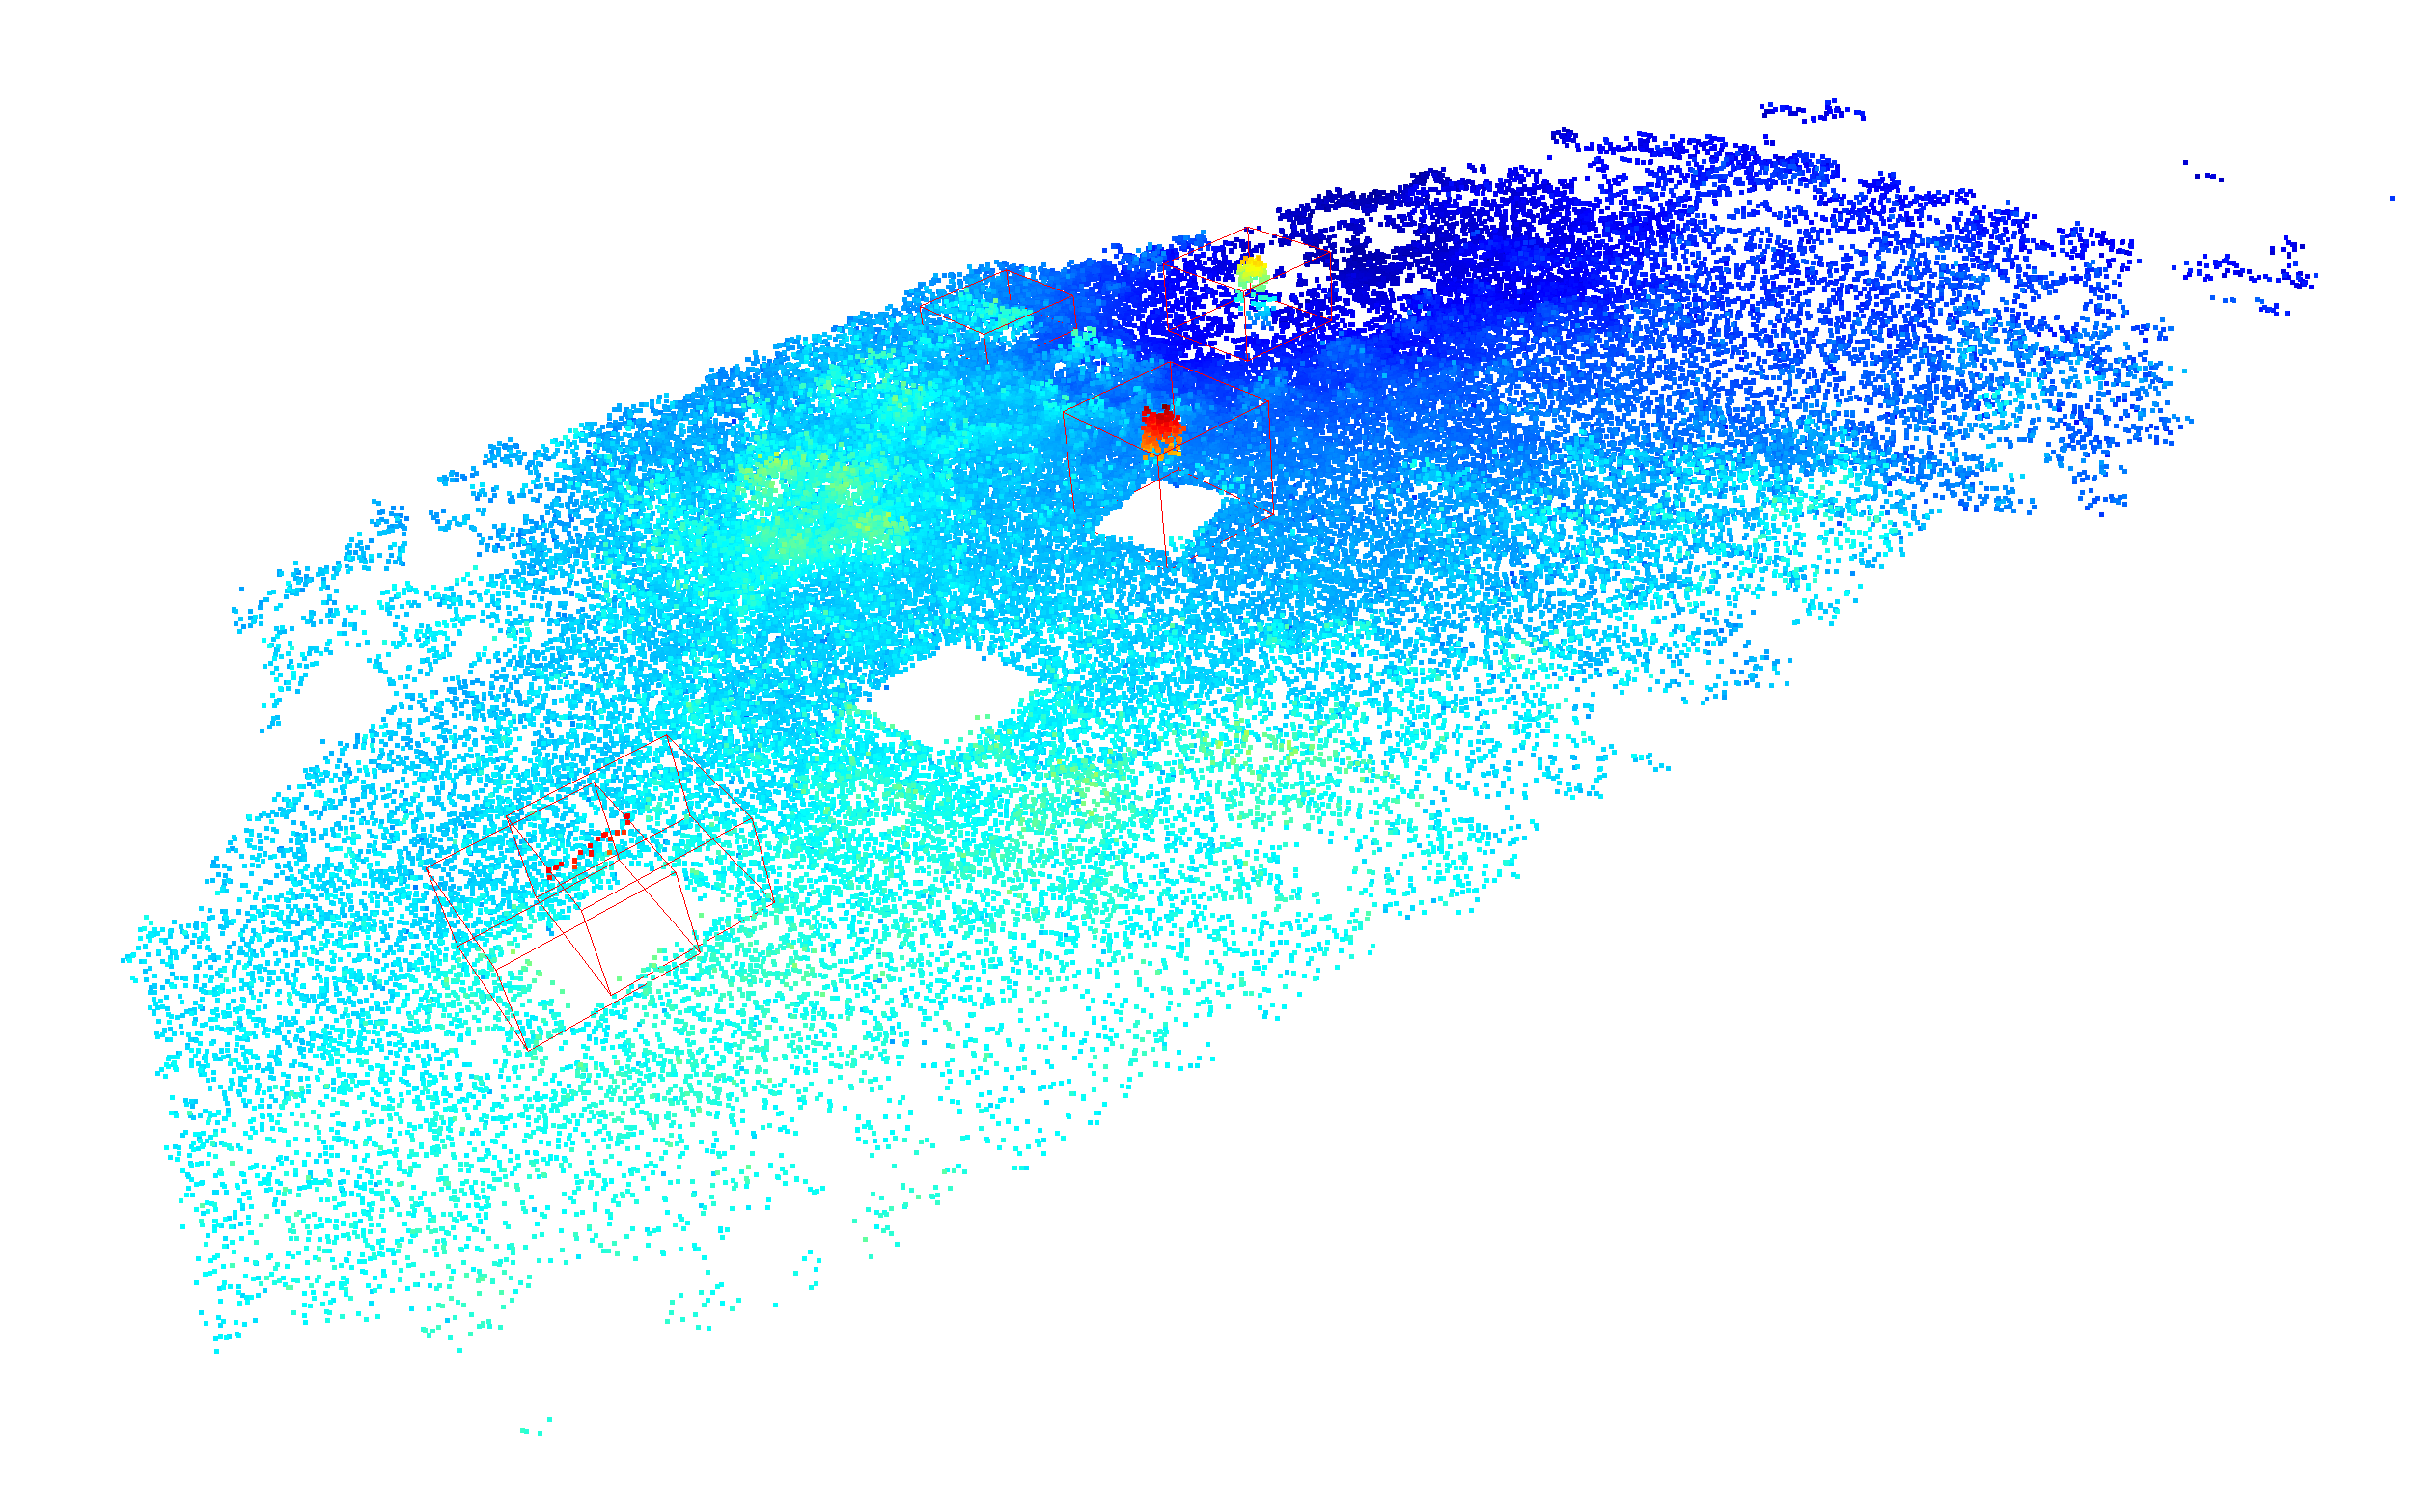
\includegraphics[width=0.45\textwidth]{images/plants_colmap.png}%
    \label{fig-plant_colmap}}
    \hfil
    \subfloat[]{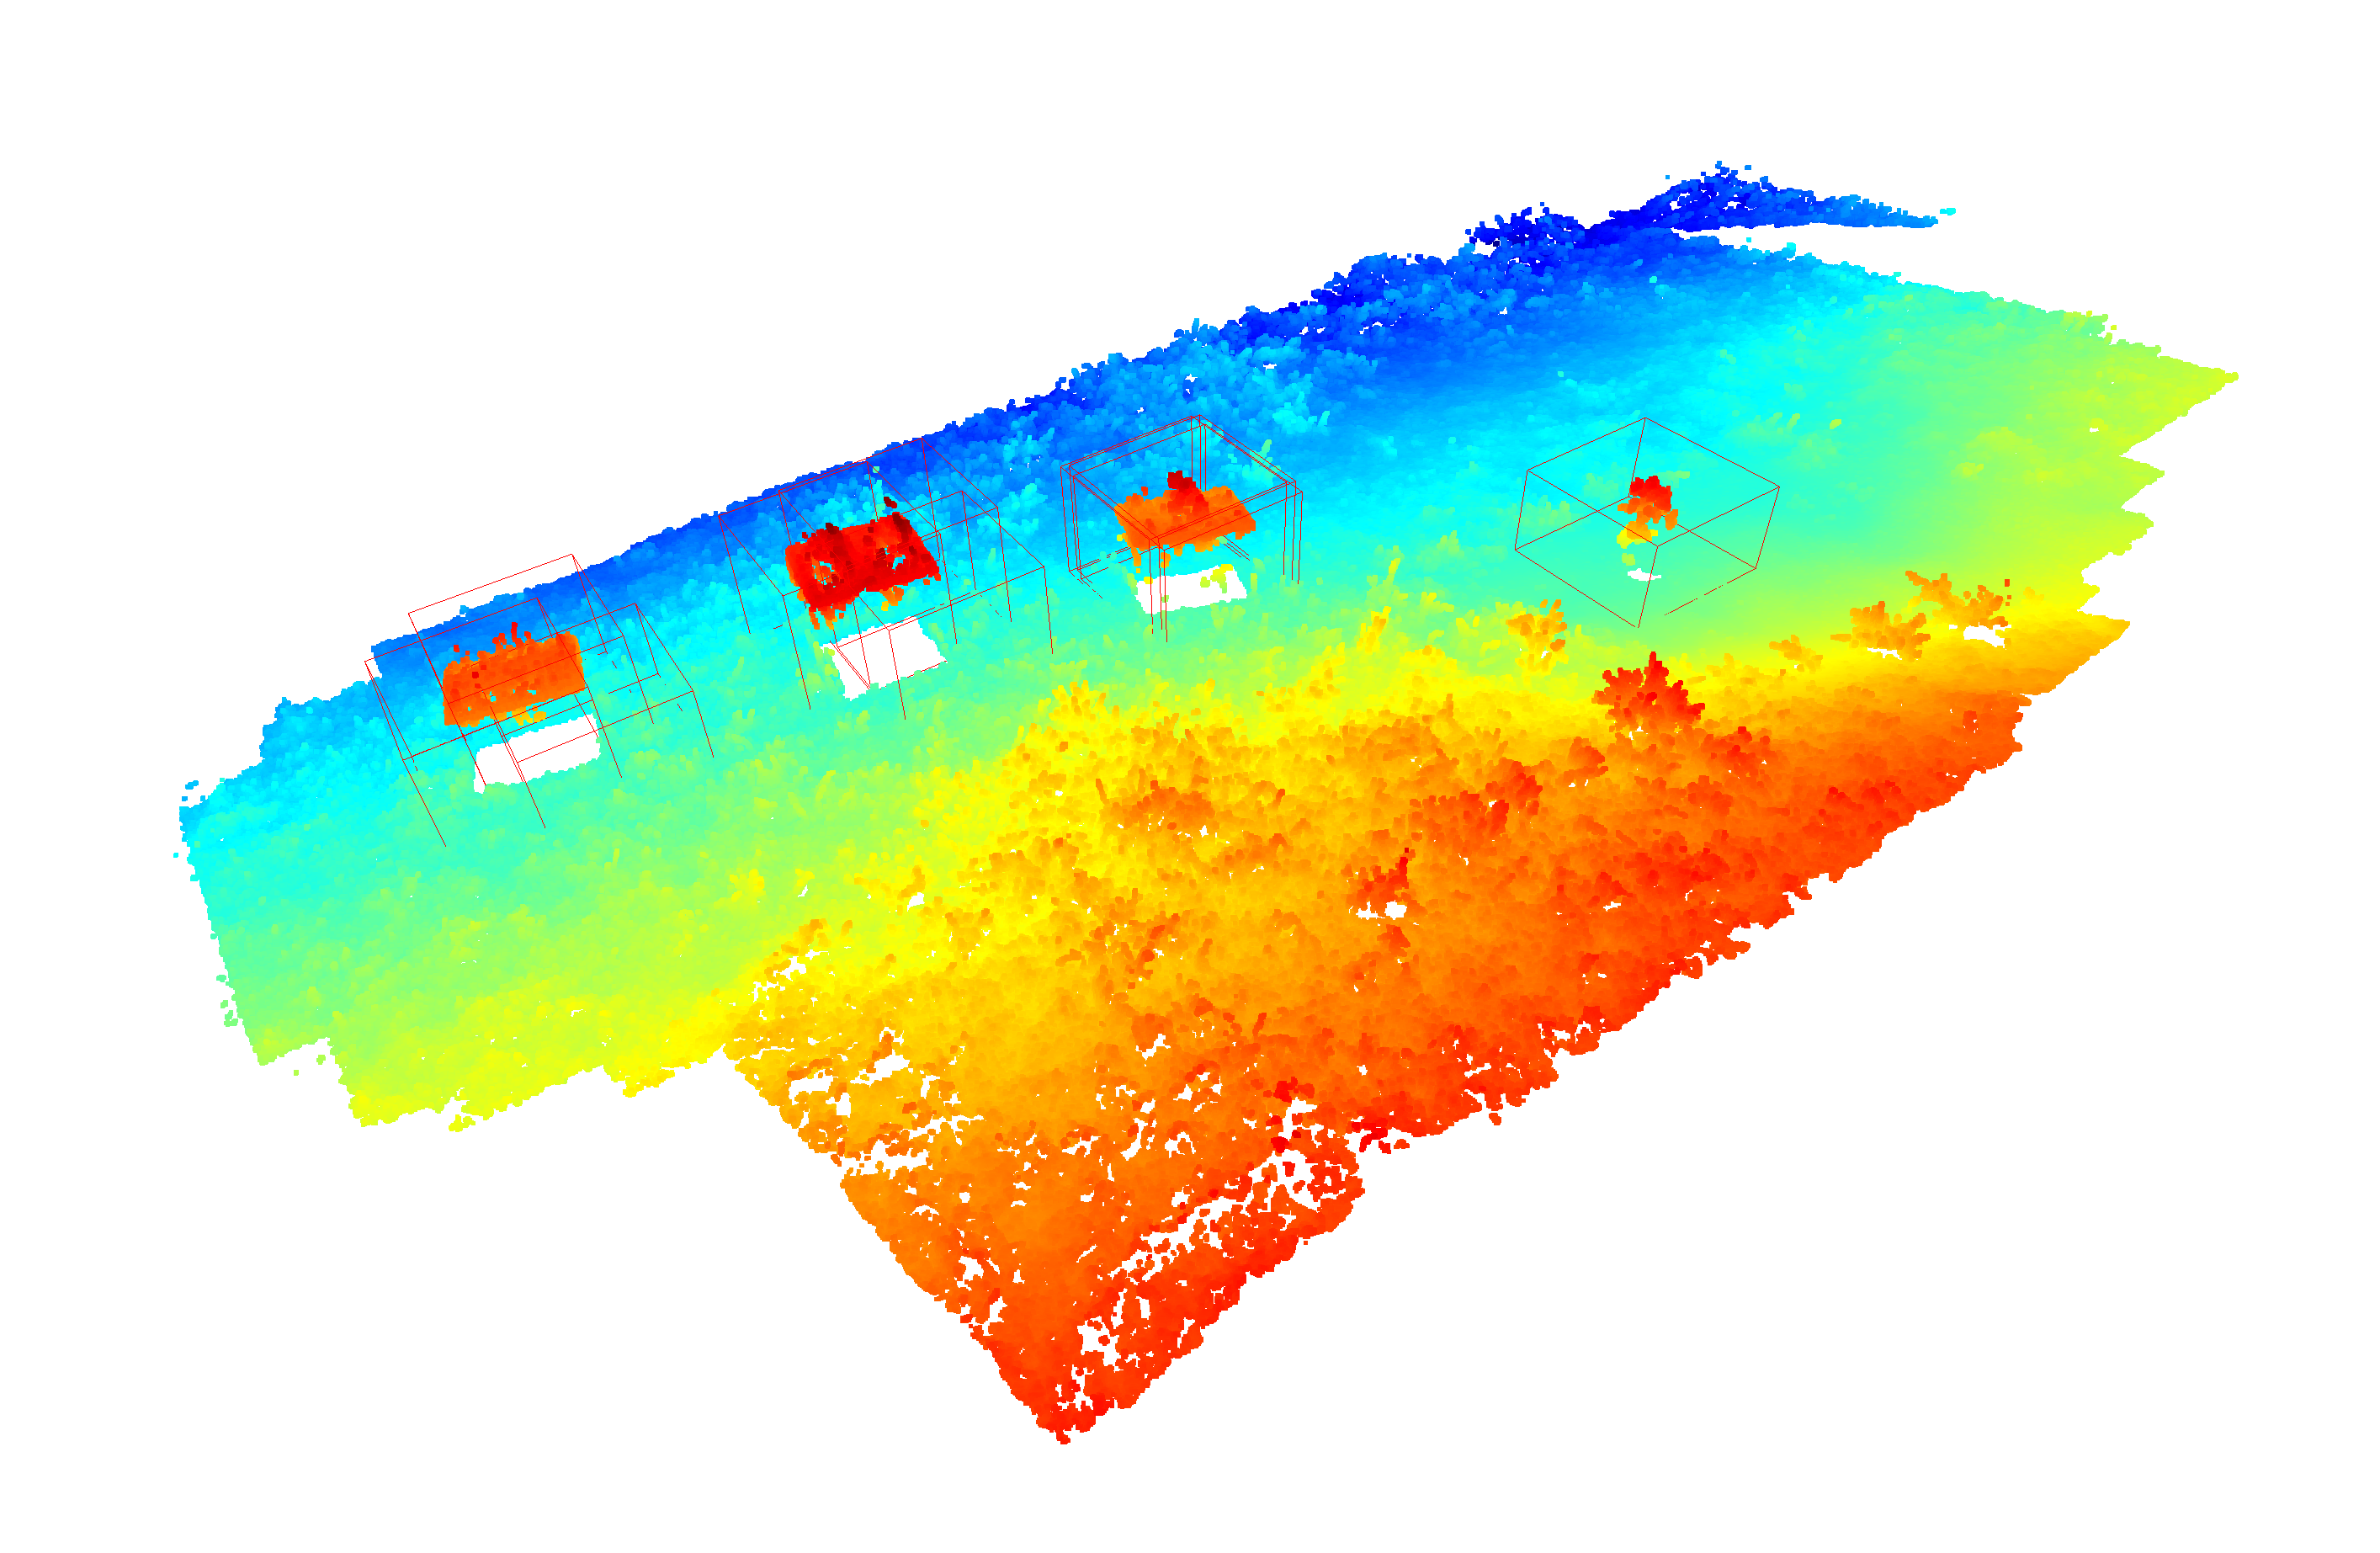
\includegraphics[width=0.45\textwidth]{images/plants_pix4d.png}%
    \label{fig-plant_pix4d}}
    \caption{The found plants represented as red bounding boxes in the point cloud. The colour of each voxel is mapped on the z-coordinate of the respective voxel. (a) is the point cloud acquired through incremental SfM (\cref{fig-colmap_clr}). (b) is the point cloud acquired through MVS in PIX4Dmapper (\cref{fig-pix4d_stereo})}
    \label{fig-plants}
\end{figure*}

\hypertarget{conclusion}{%
\section{Conclusion}\label{conclusion}}

The paper proposed a method for constructing a 3D point cloud of plants
from overhead images taken by a UAV. The incremental SfM algorithm,
processing the unordered downsampled dataset, successfully generates a
3D point cloud. A comparison with the commercially available PIX4Dmapper
revealed, that the commercial solution generates 150\% more voxels.
Furthermore, by reconstructing the point cloud with the high resolution
images, and finally applying multi-view stereo (MVS) for point cloud
densification, 950\% and 9000\% more voxels are generated respectively.

For plant determination, a peak finding algorithm is applied to the
point cloud. After filtering the point cloud for outliers, a plane is
fitted, and plants in respect to the plane searched for. A fixed
bounding box is created for each plant. Because of a missing
segmentation, the algorithm can not distinguish between plants and
surrounding points. Additionally, the fixed-size bounding boxes fail to
adapt to plant dimensions, further inducing errors.

\hypertarget{future-research}{%
\subsection{Future Research}\label{future-research}}

While this paper has provided valuable insights and advancements in the
field of 3D reconstruction through incremental SfM, there are several
points of improvements to enhance the 3D reconstruction and the plant
phenotyping itself. The comparison in Section~\ref{sec-results} showed,
that the commercial solution computes denser point clouds than the open
source implementation of the incremental SfM. To improve this,
multi-view stereo (MVS) \autocite{bailer2012} and it's refined variation
pixelwise view selection for multi-view stereo
\autocite{schönberger2016a} could be applied. However it must be noted,
that a computation of a denser point cloud has to be viewed critically,
as the computational effort rises exponentially with more voxels and
thus a trade-off between the accuracy and computational effort should be
analysed \autocite{paulus2019,li2022}.

Another way to improve point clouds while still keeping the required
computing power low, is to incorporate a RTK-GNSS signal, which provides
spatial information about a taken image. Taking the location data into
account, a stereo matching and reconstruction can be done through
calculating the baseline of two images from the location data, after
each acquired image. With this approach a real-time reconstruction can
be achieved \autocite{hasheminasab2020,matsuura2023}. To work out a more
accurate location of each image, and thus a higher accuracy baseline,
ground control points (GPC) either as physical markers in the field or
through feature matching should be investigated. Through the alignment
of each new image, the accuracy of the position, thereby of the baseline
and the stereo matching can be improved \autocite{feng2023}.

Recently 3D reconstruction through deep learning approaches like neural
radiance fields (NeRF) \autocite{gao}, which is already used in the
agricultural domain in the form of Zero NeRF \autocite{peat2022}, or
Gaussian splatting \autocite{kerbl} have gained considerable attention
for its ability to capture detailed spatial information in submillimeter
accuracy from 2D images.

After retrieving a sufficient 3D point cloud of a plant, different
approaches for phenotyping of plants should be looked into. For growth
analysis, the measurement of plant heights can be done through disparity
maps \autocite{matsuura2023}. In most cases, more information about
plants, such as width, convex hull, projected leaf area, leaf density,
number of leaves, and the respective leaf lengths can be retrieved
through deep learning segmentation. Through repeated acquisition over
time, a time variable can be induced and thus a functional structural
plant model is retrieved \autocite{paulus2019,li2022,soualiou2021}.

\newpage

\printbibliography[title=References]

\end{document}

